
\subsection{An example of Auction Design}
The idea of this part has established after discussion with Dazhong Wang and the mechanisms in this part are jointly designed by us.

We would like to design a mechanism for selling goods with  uncertain values.
Here a distribution assumption is used. Auctions are one of the most successful areas where the development of economics
theory and practice help each other. I will try to investigate this area from
a mechanism design perspective in this section. The material is put here as an example of what can be implemented for some special market. 

Here we focus on revenue maximization for the seller of an indivisible experience
good under a situation in which buyers are all ex-ante identical. The only information they all have is an identical
value distribution of the experience good. In our
setting, the seller can freely give any buyer access to get his true private value, which process we call experiencing the good. If the seller is
unable to charge experience fee, she may maximize her revenue by excluding just one buyer from experiencing, which is in conflict with the social efficiency. If
the seller is able to charge experience fee, she will maximize her revenue through setting
the price at a level such that every potential buyer will buy the experience, 
resulting in the maximal trading surplus which is fully extracted by the seller.

Of course, the equilibrium of implementation in such a mechanism is ex ante,  the following chapter will be concerned with ex post implementation.

Now the details are as follows. A seller(she) has a single indivisible good, and wants to sell the good to a group of $N$ buyers indexed by $i=1, 2, . . . , N$(buyers and
bidders are used interchangeably in this paper, and are assumed to be
male). All parties are risk neutral. 
 The value of retaining the good to the seller
is publicly known as $\underline{v}(\geq 0)$ in this paper. Bidder i's valuation of the object
is $v_{i}$, and $v_{i}$ has independent identical distribution $F(x)$ with support $[\underline{v}, \overline{v}]$, 
where $\overline{v}>\underline{v}$, and $\overline{v}=+\infty$ is allowed. 
In the beginning, no one can directly observe the $v_{i}$. Only the distribution is common knowledge among all the parties. However, if the seller gives a chance of experiencing the good to a buyer, the buyer can learn of his $v_{i}$ after experiencing. 
 

The seller designs a sales mechanism to sell the
good. The sales mechanism consists of two stages, the experience stage, and the auction stage. 
After the experience stage, the seller will allow those who
have experienced the good to
participate the auction. By Revenue Equivalence Principle, we analyze the case that the seller chooses the second-price
sealed-bid auction in the auction stage without loss of generality. In the auction stage, if no bidder bids a value exceeding a reserve price
, then the good is sold to the unexperienced buyer at the
price $\mu$(the expectation of v) when there is an unexperienced buyer. Here we assume that the buyer will choose to buy the good if he is indifferent between buying and not buying the good. 
The timeline is shown in the Figure 1. 
\begin{figure}
\begin{center}
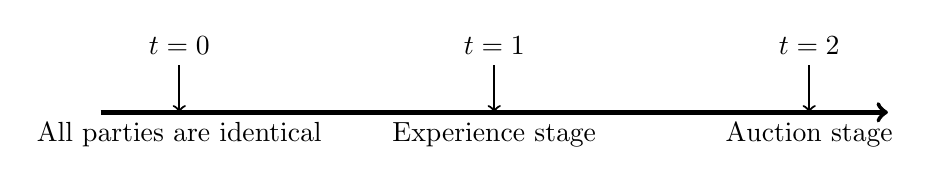
\begin{tikzpicture}
 \draw[->, ultra thick] (5, 0) -- (15, 0);
 \draw[->, thick](6, 0. 6)node[above]{$t = 0$} -> (6, 0)node[below]{All parties are identical } ;
 \draw[->, thick](10, 0. 6)node[above]{$t = 1$} -> (10, 0)node[below]{Experience stage};
 \draw[->, thick](14, 0. 6)node[above]{$t = 2$} -> (14, 0)node[below]{Auction stage} ;
 \end{tikzpicture}
\end{center}
 \caption{Timing of experience good auction }
\end{figure}

\subsubsection{Setting Reserve price to extract trade surplus}
In the situation that the seller cannot charge fee for experiencing the good, 
the seller will set a reserve price in the auction stage to maximize the
revenue in a second-price sealed-bid auction. 
\begin{lemma}\label{lem}
 The hazard rate function associated with the distribution F is
defined as $\lambda(x) = f(x) / (1 - F(x))$. The optimal reserve price $r$ satisfies $r - 1/\lambda(r)= v^*$. The $v^*$ denotes the seller's reserve revenue/valuation. 
\end{lemma}
\begin{proof}
Let $R(r, m)$ denote the revenue of the seller when the reserve price is $r$ and the number of buyers experiencing the good is $m$. 

Obviously, $r$ should be higher than $v^*$ to have an effect of enhancing the price. 
Then the expected value of seller revenue can be calculated as the sum of three parts, the revenue from the auction when the second highest bid is above the reserve price $r$, the revenue from the auction when the highest bid is above the reserve price but the second highest price is below the reserve price $r$, and the reserve revenue/valuation$v^*$ when the highest bid is below the reserve price $r$. 
\begin{equation}\label{equ}
R(r , m) =\int_{r}^{\overline{v}}x\mathrm{d}G_{(2)}^{m}(x) + rmF^{m-1}(r)[1 - F(r)] + v^* F^{m}(r)
\end{equation}
where $G_{(2)}^{m}(x) = F^{m}(x) + mF^{m-1}(x)[1 - F(x)]$. 


Differentiating this with respect to $r$ and simplify, we obtain
$$-rmF^{m-1}f(r)+mF^{m-1}(r)(1-F(r))+v^* mF^{m-1}(r)f(r)$$

The first order condition is 
$$r^* - \frac{1 - F(r^*)}{f(r^*)} = v^*$$
\end{proof}
\begin{remark}
 Under regularity conditions, the first order condition is also sufficient for optimality. 
\end{remark}
 If the seller gives a buyer the chance to experience the good, no buyer will refuse since experiencing the good means some chance
of gain. Thus the number of buyers who can experience the good is at her control. Intuitively, she 
wants to obtain a high revenue from the auction by letting more buyers to experience as long as there is still an unexperienced buyer, for the seller can sell the good to him
at price $\mu$ when no bidder bids over the
reserve price. This is summarized in the following proposition. 
\begin{prop}
 As the number m of buyers experiencing the good increases, the expected value of seller revenue increases as long as $m\leq n-1$. 
\end{prop}
\begin{proof}
When the reserve revenue $v^*$ is obtained by selling the good to a 
unexperienced buyer, $v^*=\mu$. Then by equation~\ref{equ} in the proof of Lemma~\ref{lem}, 
\begin{equation}
R(r, m) = \int_{r}^{\overline{v}}x\mathrm{d}G_{(2)}^{m}(x) +
rF^{m-1}(r)[1 - F(r)] + \mu F^{m}(r)
\end{equation}
where $G_{(2)}^{m}(x) = F^{m}(x) + mF^{m-1}(x)[1 - F(x)]$. 

When $m\leq N-1$, the best reserve price is $r=r^*$ which is the solution to $r^*-1/\lambda(r^*)=\mu$. The revenue is $R(r^*, m)$. 
 By the first order stochastic dominance, it is straightforward to show $R(r^*, m) > R(r^*, m')$ for any $N-1\geq m>m'$. 
\end{proof}
However, letting $N$ potential buyers to all experience the good may
not be better than just letting $N-1$ buyers to experience. Because the former may let go the
safe option of selling the good at $\mu$. Indeed, it depends on the
distribution F(x). A careful research of us has led to the following conclusion. 
\begin{thm}
 The seller does not always want all buyers to experience the good under the setting here. 
 \end{thm}
 \begin{proof}
 When every buyer has experienced the good, then by lemma~\ref{lem}, 
 the reserve price should now be set to $\hat{r}$, which is the solution to $\hat{r}-1/\lambda(\hat{r})=\underline{v}$, since the reserve
valuation is $\underline{v}$ and the revenue 
is $R(\hat{r}, N)$ using equation~\ref{equ}. 
Generally speaking, 
 $R(\hat{r}, N)<R(r^*, N-1)$ for many distributions and the potential buyers' number N. 
 \end{proof}
Figure 2 shows the values of $R(r^*, N-1)-R(\hat{r}, N)$ for different
values of parameters in Beta distribution(with the horizontal axis denoting N). 
\begin{figure}
\centering
\includegraphics[width = 11cm]{betaGraph.pdf}
\caption{Difference in revenue: $R(r^*, N-1)-R(\hat{r}, N)$} \label{fig:graph}
\end{figure}

\begin{remark}
 Specially for the uniform distribution, we have, when $N\leq 7$, $R(\hat{r}, N)<R(r^*, N-1)$. 
\end{remark}

\subsubsection{Charging Experience fee to extract trade surplus}
 We then consider the case where the seller can charge experience fee. For the seller, at the experience-stage, how to optimally set price of exprience? 
If a certain number of buyers are permitted to experience the good, each of those buyers is supposed to get a nonnegative ex ante expected payoff from participating the
subsequent second-price auction. Suppose that buyers will buy the experience when they are indifferent between remaining
uninformed and buying the experience to be informed. 
 Then the seller should set the price equal to a buyer's ex ante expected payoff of participating the auction to extract all the expected trade surplus. Intuitively, the ex ante expected payoff of experiencing buyers depends on the number of auction partipants. 
%First, we set the prespecified price as $\mu$ for the auction. Then the expected result of the auction can be calculated. \end{comment}



Next, we will offer the formula for the experience fee in the following lemma. 
\begin{lemma}
 The experience fee $P(m)$ can be formulated as 
\begin{equation}
 P(m) = \begin{cases}\int_{\mu}^{\overline{v}}\int_{\mu}^vF^{m-1}(t)\mathrm{d}tf(v) \mathrm{d} v, &\textrm{if}\quad m \leq N-1\\
\int_{\underline{v}}^{\overline{v}}\int_{\underline{v}}^v F^{N-1}(t)\mathrm{d}tf(v) \mathrm{d} v, &\textrm{if}\quad m = N
\end{cases}
\end{equation}


\end{lemma}
\begin{proof}
 When there are $m(\leq n-1)$ buyers knowing one's own value information, the value of the information is
\begin{align*}
P(m)&= \int_{\mu}^{\overline{v}}(\int_{\mu}^v (v-t)\mathrm{d}F^{m-1}(t)+(v-\mu)F^{m-1}(\mu))f(v)\mathrm{d}v \\
&= \int_{\mu}^{\overline{v}}\int_{\mu}^vF^{m-1}(t)\mathrm{d}tf(v)\mathrm{d}v
\end{align*}

$P(N)$ can be formulated as, 
 \begin{align*}
P(N) &= \int_{\underline{v}}^{\overline{v}}\int_{\underline{v}}^v(v-t)\mathrm{d}F^{N-1}(t)\mathrm{d}tf(v)\mathrm{d}v \\
 &= \int_{\underline{v}}^{\overline{v}}\int_{\underline{v}}^v F^{N-1}(t)\mathrm{d}tf(v)\mathrm{d}v
\end{align*}
\end{proof}

\begin{lemma}
As the number of buyers knowing one's own value information increases, the expected value of knowing one's own value information decreases. 
\end{lemma}
Notice that for many distributions and potential buyers' number n, $P(N) < P(N-1)$. In such cases, the seller set price at $P(N)$, and 
the buyers' domininant stratey is to buy the experience. 
Since every buyer knows the true value in the auction and expected gain of every buyer is zero now, the seller can extract full surplus through setting appropriate experience fee. the 
social surplus is maximized and fully extracted by the seller. 



The above reasoning leads to the following conclusion

\begin{thm}

 If the seller can charge fee for letting one buyer know his true value, then the seller will set the price
 $ \int_{\underline{v}}^{\overline{v}}\int_{\underline{v}}^v F^{n-1}(t)\mathrm{d}tf(v)\mathrm{d}v$ to fully extract all the surplus of trade, and the revenue she get is 
 \begin{equation}
 E(V_{(1)}^N)=\int_{\underline{v}}^{\overline{v}} x\mathrm{d}F^N(x) 
 \end{equation}
where $V_{(1)}^N$ denotes the highest bid. 
\end{thm}
 This is the best possible result for the seller, maximizing the trade surplus and minimizing all the buyers' share. 


The example is supposed to shed light on a seller's optimal
sales mechamism design when buyers have identical value distribution about the
experience good, but do not know the private value before the experience. The seller controls the number of buyers to experience. 

When the seller is not able to charge experience fee, her optimal sales mechanism might be to exclude a buyer from experiencing the good, which harms social
 efficiency. When the seller is allowed to charge fee, the result is efficient. However, the defect is that
 all the trade surplus is extracted by the seller. 